% Created 2018-04-06 Fri 16:21
\documentclass[11pt]{article}
\usepackage[utf8]{inputenc}
\usepackage[T1]{fontenc}
\usepackage{fixltx2e}
\usepackage{graphicx}
\usepackage{longtable}
\usepackage{float}
\usepackage{wrapfig}
\usepackage{rotating}
\usepackage[normalem]{ulem}
\usepackage{amsmath}
\usepackage{textcomp}
\usepackage{marvosym}
\usepackage{wasysym}
\usepackage{amssymb}
\usepackage{hyperref}
\tolerance=1000
/home/hmshen/dotfiles/latex/orgconfigs.tex
\author{Haoming Shen}
\date{04/02/2018}
\title{Documentation on Solar Forecasting Project}
\hypersetup{
  pdfkeywords={},
  pdfsubject={},
  pdfcreator={Emacs 24.5.1 (Org mode 8.2.10)}}
\begin{document}

\maketitle
\tableofcontents

\clearpage

\section{Overview}
\label{sec-1}
This project aims at improving intra-day Ground Horizontal Irradiance
(GHI) forecasting using machine learning based algorithms. Predicting
the amount solar energy in the next few hours/days is of great
importance to power system operations and control. Currently two
methods are implemented and documented below. If you have any
questions with respect to this project, please contact me through
email (my unique name is `hmshen`)

NOTICE: If you need to use the code below (even part of it), I would
recommend you read it critically before using it.

\subsection{Github repo for this project}
\label{sec-1-1}
\url{https://github.com/hm-shen/weather_forecast/tree/master/src}

\subsection{Dependencies}
\label{sec-1-2}
Tensorflow, Sklearn, Pandas, Numpy, Scipy, \ldots{}.

I would recommend you use Anaconda Python.

\section{SVM Based Solar Irradiance Forecasting}
\label{sec-2}

\section{LSTM Based Cloud Fraction Forecasting}
\label{sec-3}
Since both hourly GHI and hourly cloud fraction can be considered as
time series, solving it using Long short-term memory (LSTM) becomes
natural. This part implements a simple LSTM model for supervised cloud
cover and GHI forecasting.

\subsection{Getting Started}
\label{sec-3-1}
To perform cloud fraction prediction on NREL data sets, please run the
following command from folder \texttt{cloud\_forecasting/src/}:

\begin{verbatim}
python -p /path/to/NREL_data/ \
       -f 'average or variance' \
       -o /path/to/output/ \
       -c /path/to/configuration file/ \
       -n 'name of the dataset' \
\end{verbatim}

Several example bash scripts are included in \texttt{/src} folder.

\subsection{Implementation}
\label{sec-3-2}
Note that this implementation of LSTM based time series is based on
\url{https://github.com/tgjeon/TensorFlow-Tutorials-for-Time-Series}

\subsubsection{Overall Framework of LSTM}
\label{sec-3-2-1}
\href{http://colah.github.io/posts/2015-08-Understanding-LSTMs/}{Tutorial on LSTM model can be found here (click me!)}

All diagram of the architecture is shown below

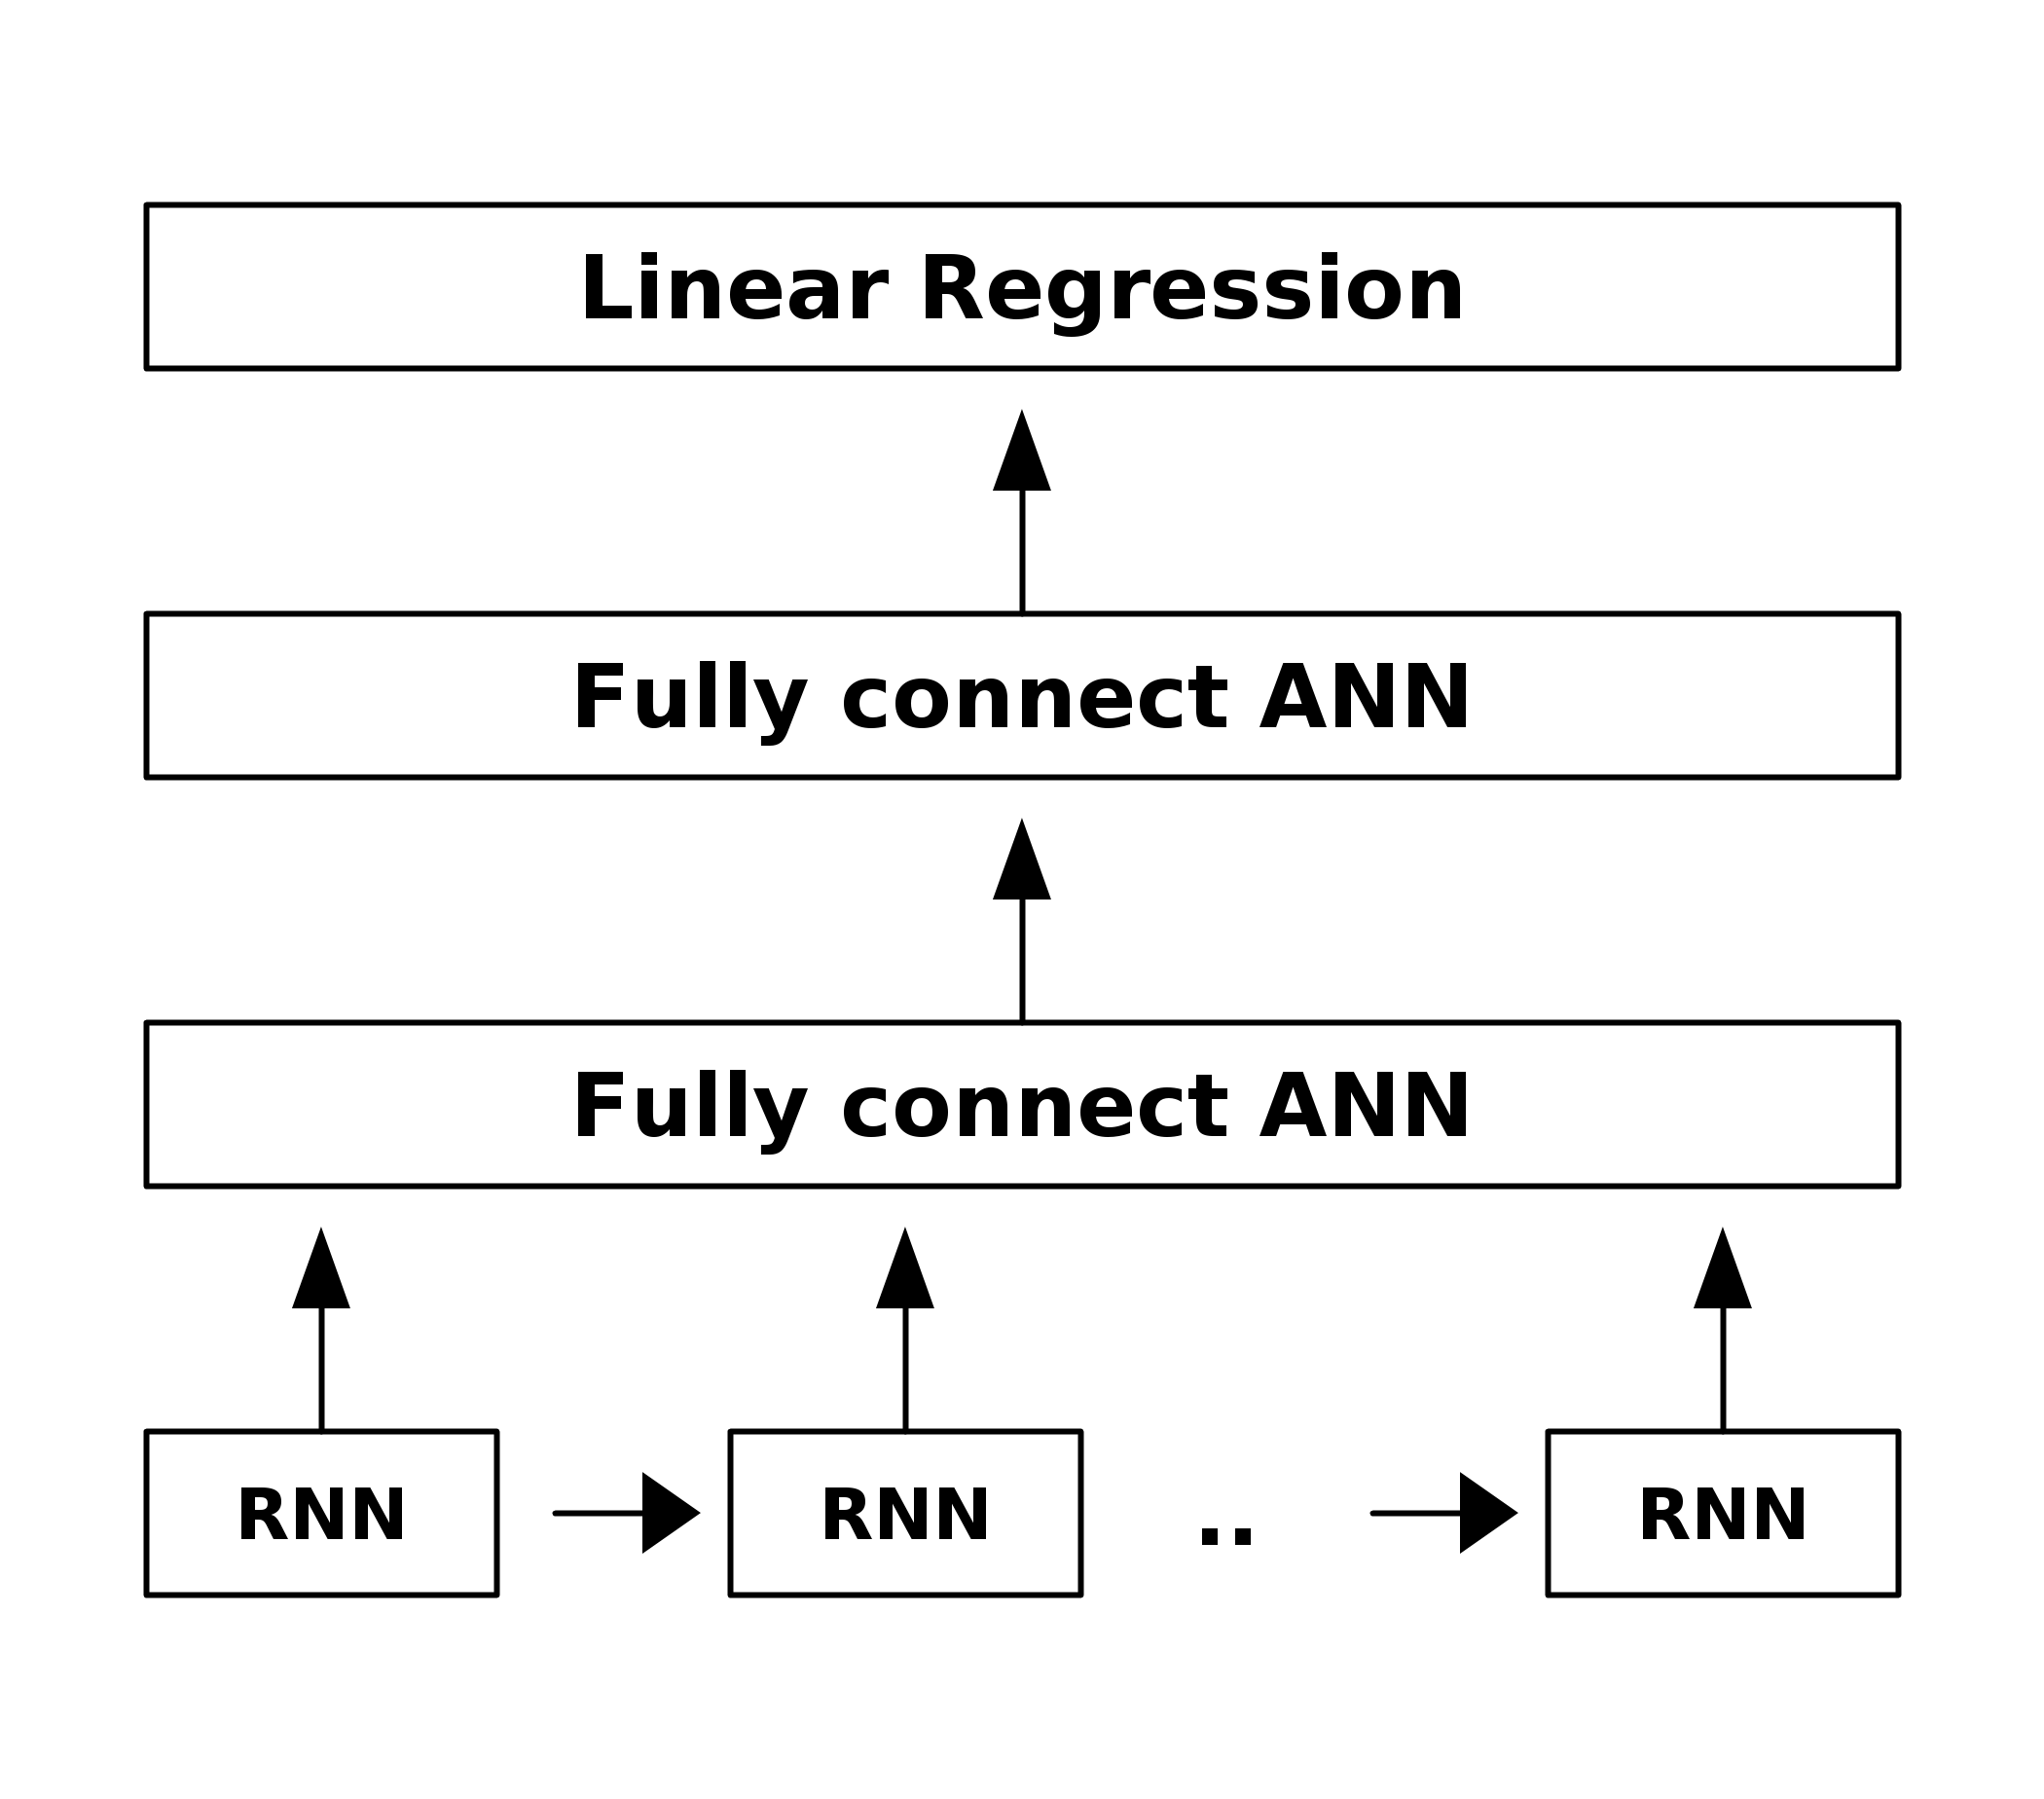
\includegraphics[width=.9\linewidth]{LSTM-Structure.png}

where the LSTM cell is represented as "unrolled" RNN cells. So for
each input \(x_t\), \(y_t\) will be generated by LSTM cell and feed
into two layers of fully connected artificial neural networks
(ANN). Then the output is used as the input to a linear regressor.
\subsubsection{Parameters}
\label{sec-3-2-2}

Parameters for LSTM are listed below:
\begin{table}[htb]
\caption{Parameters for setting up LSTM}
\centering
\begin{tabular}{ll}
\toprule
Parametter & Description\\
\midrule
time steps & how many time steps is used to predict (features)\\
rnn layers & the configuration of rnn layers using a list of dict\\
dense layers & number of units in each dense layer\\
\bottomrule
\end{tabular}
\end{table}

\subsection{Some details on data preprocessing}
\label{sec-3-3}
Those NREL data contained in the \texttt{data/} folder is a little bit messy
in the sense that there may be invalid cloud fraction data in each day
(e.g. \texttt{nan}, \texttt{-1}). Thus, to remove days with too many messy data,
there are two variables, \texttt{ubd\_min}, \texttt{lbd\_max}, responsible for
removing all invalid days: all days where the first valid data
appearing later than \texttt{ubd\_min} is removed; similarly, all days where
the last valid data appearing before \texttt{lbd\_max} is removed. This way,
we select days with number of valid data at least (\texttt{lbd\_max} -
\texttt{ubd\_min}). Also note that these two variables are related to the data
set you are using and thus should be set by hand in the source code
\texttt{/src/driver.py}.
% Emacs 24.5.1 (Org mode 8.2.10)
\end{document}
